Tutkimuksissa \parencite{RahmanAkond2019TSSS}, \parencite{RahmanAkond2021SSiA} käytettiin
tutkimuksia varten tehtyjä työkaluja, jotka oli empiirisesti validoitu toimiviksi.
Kyseiset työkalut eivät yleisesti ole tiedossa tai käytettävissä. Tässä kappaleessa on
kuitenkin esitelty yksi työkalu, ansible-lint, joka edes auttaa havaitsemaan vastaavia
virheitä ja johon on mahdollista rakentaa itse lisätarkistuksia \parencite{SestoVincent2020ATaV}.

\section{Ansible-lint}

Ansible-lint on työkalu, joka on suuniteltu tarkistamaan noudatetaanko parhaita
käytäntöjä ja sen myötä edesauttamaan käytäntöjen parantamista \parencite{GithubAnsibleLint}.
Työkalua ei ole nimenomaan suuniteltu huomaamaan turvallisuuspuutteita, mutta parhaat
käytännöt sisältävät myös asioita, jotka ovat turvallisuuden kannalta oleellisia.

\subsection{Manuaalinen ajaminen}

Ansible vaatii ajamiseen tarkoitetulla palvelimella python3.8:n \parencite{AnsibleDocs}.
Tämän myötä koneelle on todennäköisesti asennettu myös pip. Työkalun asentaminen
onnistuukin tällöin helposti pip:in avulla \parencite{AnsibleLintReadTheDocs}:

\begin{lstlisting}[
    basicstyle=\small,
    label={lst:install-ansible-lint},
    language=bash
]
    $ pip3 install ansible-lint
\end{lstlisting}

Työkalu ei tarvitse lisämäärityksiä vaan voi tunnistaa automaattisesti tarvittavat
tiedostot ansible-projektista \parencite{AnsibleLintReadTheDocs}:

\begin{lstlisting}[
    basicstyle=\small,
    label={lst:run-ansible-lint},
    language=bash
]
    $ ansible-lint
\end{lstlisting}

Komennon antama ulostulo voi näyttää esimerkin \ref{lst:ansible-lint-simple-example} mukaiselta.

\begin{lstlisting}[
    basicstyle=\small,
    label={lst:ansible-lint-simple-example},
    breaklines=true,
]
    no-handler: Tasks that run when changed should likely be handlers
    hcloud_roles/hcloud_server/tasks/main.yml:119 Task/Handler: Discord notification

    risky-file-permissions: File permissions unset or incorrect
    roles/address_checker/tasks/main.yml:13 Task/Handler: DB volume directory
\end{lstlisting}

Kattavampi ulostulo on esitelty liitteessä \ref{lst:ansible-lint-example}.

\subsection{Automaattinen ajaminen Gitlab CI:n avulla}

Gitlabia tietovarastona (repository) käyttävät ohjelmistoprojektit voivat käyttää
jatkuvan integraation suorittamiseen Gitlab CI/CD:ta. Gitlab CI/CD perustuu
avoimeen lähdekoodiin ja sen ilmainen versio on ollut jo aikoinaan parhaimpia ja
kattavampia. \parencite{alma9911268330505973}

Yleisesti tunnettuja vaihtoehtoisia ratkaisuja ovat muun muassa Github Actions,
Travis CI, CircleCI ja Jenkins.

Gitlab CI:ssa tarvittavat määritykset laitetaan `.gitlab-ci.yml`-tiedostoon
\parencite{GitlabCICDDocs}. Esimerkissä \ref{lst:gitlab-ci-ansible-lint} esitelty
yksinkertainen vaihtoehto, jolla saadaan ajettua `ansible-lint` automaattisesti
jokaisen muutoksen myötä.

\lstinputlisting[
    basicstyle=\small,
    caption={Esimerkki yksinkertaisesti Gitlab CI määrityksestä ansible-lint:n ajamiseen automaattisesti},
    label={lst:gitlab-ci-ansible-lint},
]{code/gitlab-ci-ansible-lint.yaml}

Ylläoleva esimerkki on yksinkertainen eikä sisällä esimerkiksi välimuistin
määrittämistä, jotten työkaluja tarvitse jokaisella suorituskerralla asentaa
uusiksi. Lisäksi työkalun ajaminen joka ei kerta ei välttämättä ole suositeltava
ratkaisu.

\subsection{Tulosten näyttäminen Gitlabissa}

Gitlab CI vertailee koodinlaatu raportteja eri haarojen välillä ja näyttää
tulokset merge requesteissa \parencite{GitlabCICDDocs}. Kuvassa on
näytetty esimerkki siitä, kun koodinlaatu paranee muutosten myötä.

%\begin{subfigure}{0.49\textwidth}
\pdftooltip{
    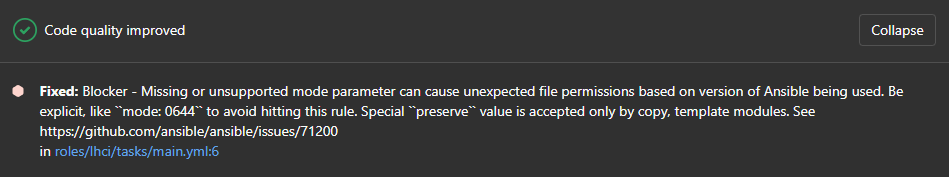
\includegraphics[
        width=\textwidth
    ]{figures/gitlab-code-quality-improved.png}}
{Kuva. Koodinlaadun parantuminen tehtyjen muutosten myötä.}
\caption{test}
%\end{subfigure}

On hyvä huomioida, että kohdehaarassa tulee olla muodostettu vastaava
raportti vähintään kerran, jotta vertailua voidaan suorittaa. \parencite{GitlabCICDDocs}

Ansible-lintin muodostavat codeclimate raportit on mahdollista ladata myös
erikseen Gitlab CI/CD Pipelinejen artifakteista. \parencite{GitlabCICDDocs}
